
\subsubsection{10.10.14}

\begin{enumerate}
	\item The time of beginning and ending of the meeting:
	18:30 - 21:40
	\item Purposes of the meeting:
	\begin{enumerate}
	  \item To choose the optimal diameter of the crossbars.
	  
	  \item To cut the aluminum profile into segments of desired length. To drill the holes in the segments and to install them between the rails.
	  
    \end{enumerate}
	\item Work that has been done:
	\begin{enumerate}
	  \item The belt for extracting the lift was bought.
	  
	  \begin{figure}[H]
	  	\begin{minipage}[h]{0.2\linewidth}
	  		\center  
	  	\end{minipage}
	  	\begin{minipage}[h]{0.6\linewidth}
	  		\center{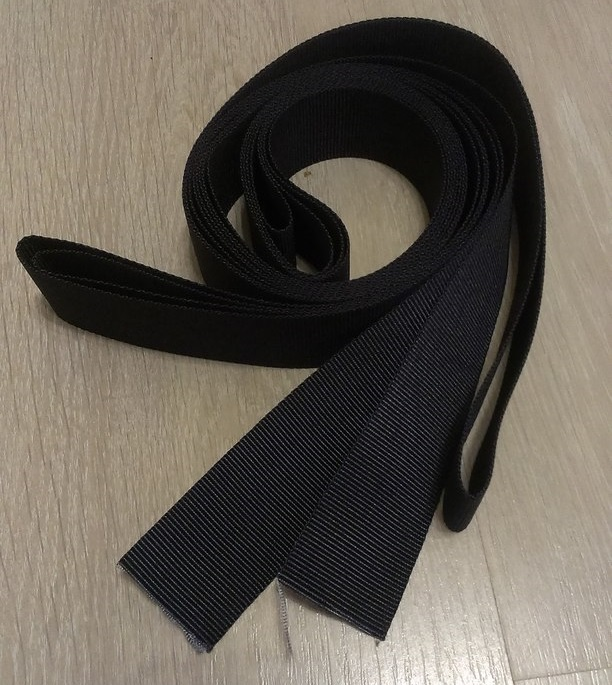
\includegraphics[scale=0.3]{days/10.10.14/images/01}}
	  		\caption{Belt}
	  	\end{minipage}
	  \end{figure}
      
      \item  It was bought aluminum strip with dimensions 200 x 5 x 0.2 cm for creation mounts of crossbars.
      
      \item It was reviewed 2 variants of crossbars: cylindrical rollers 15 mm diameter and axis diameter 5 mm from the Tetrix set. It was decided to use the axles because they are more compact.
       
      \item The axis of the smaller diameter has a cut edge. It could prevent the movement of the belt. So it was decided to impose the  sleeve on the axis. Preliminary tests demonstrated the viability of the idea.
        
      \item After that it was decided to take action:
      \begin{enumerate}
      	\item The guides of the lift were previously disassembled.
      	
      	\item  Aluminum strip was cut into 6 piecies: 2 to 30 cm and 4 to 35 cm.
      	
      	\item When we were drilling details some troubles appeared. All drills were ground off. It was decided to buy a new drill.
      	
      	\begin{figure}[H]
      		\begin{minipage}[h]{0.2\linewidth}
      			\center  
      		\end{minipage}
      		\begin{minipage}[h]{0.6\linewidth}
      			\center{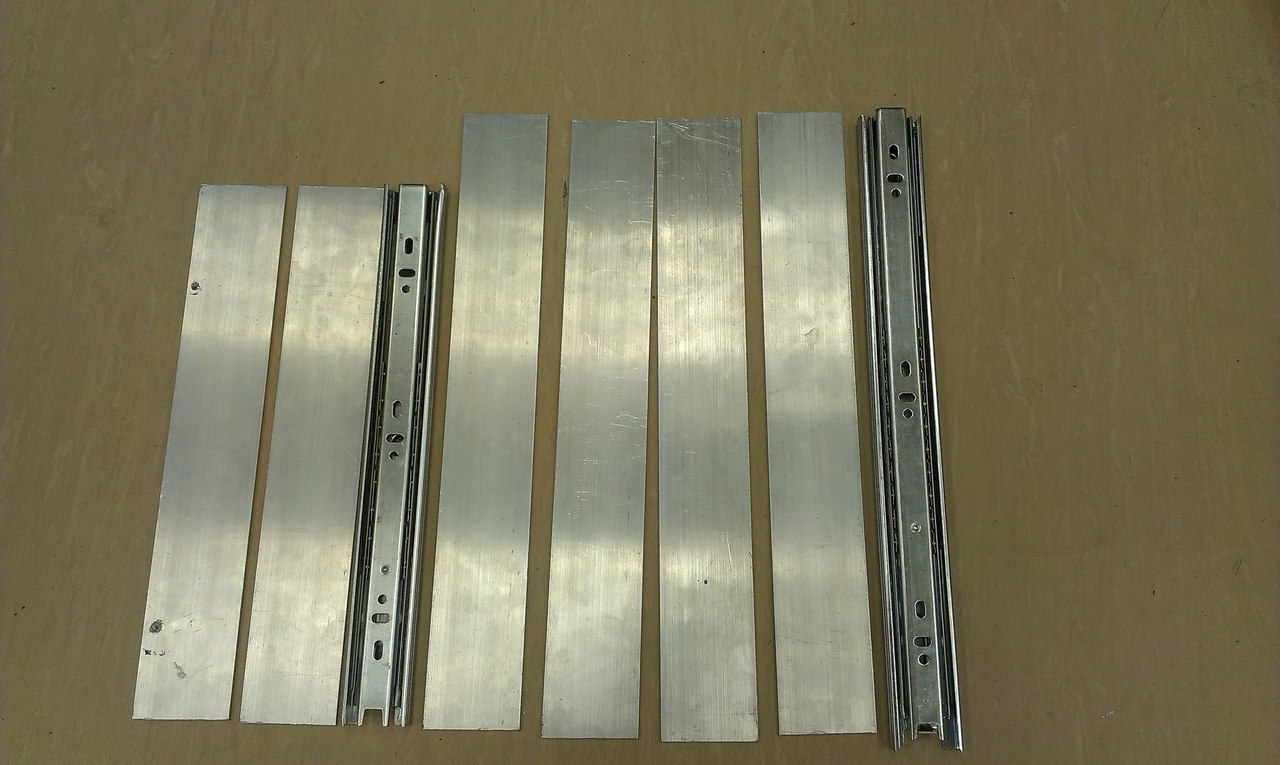
\includegraphics[scale=0.2]{days/10.10.14/images/02}}
      			\caption{Aluminum strip was cut into 6 portions}
      		\end{minipage}
      	\end{figure}
      	
      \end{enumerate}
      
    \end{enumerate}
    
	\item Results:
	\begin{enumerate}
	  \item Tracks for the lift were choosed.
	  
	  \item Beam have sawed into segments of desired length.
	  
	   
    \end{enumerate}
    
	\item Tasks for the next meetings:
	\begin{enumerate}
	  \item To buy the new drill for metal.
	  
    \end{enumerate}     
\end{enumerate}
\fillpage
